\section{test.cpp File Reference}
\label{test_8cpp}\index{test.cpp@{test.cpp}}
{\tt \#include $<$iostream$>$}\par
{\tt \#include $<$fstream$>$}\par
{\tt \#include \char`\"{}data\-In.h\char`\"{}}\par


Include dependency graph for test.cpp:\begin{figure}[H]
\begin{center}
\leavevmode
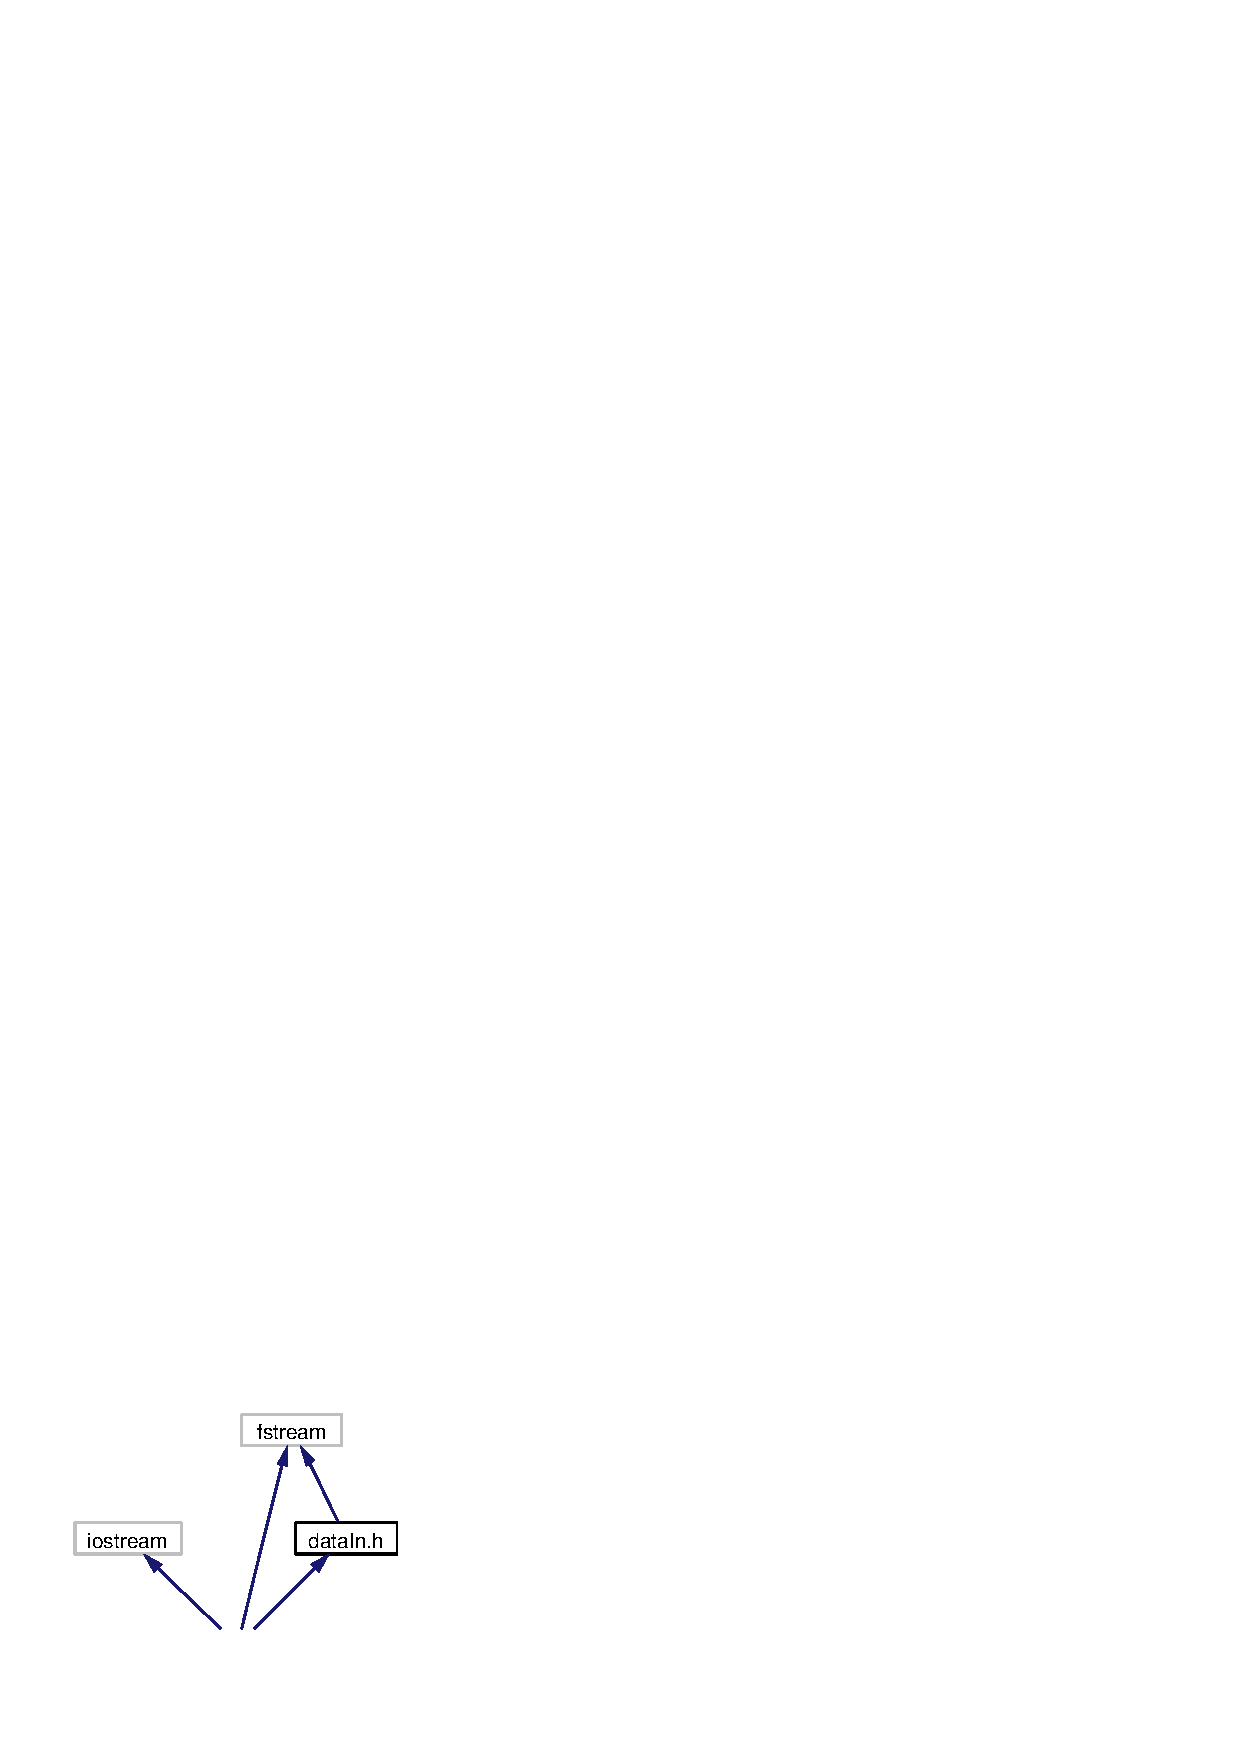
\includegraphics[width=95pt]{test_8cpp__incl}
\end{center}
\end{figure}
\subsection*{Functions}
\begin{CompactItemize}
\item 
int {\bf main} ()
\end{CompactItemize}


\subsection{Function Documentation}
\index{test.cpp@{test.cpp}!main@{main}}
\index{main@{main}!test.cpp@{test.cpp}}
\subsubsection{\setlength{\rightskip}{0pt plus 5cm}int main ()}\label{test_8cpp_a0}




Definition at line 7 of file test.cpp.

References Data\-In::name\-Of, Data\-In::Read\-Chars(), and Data\-In::Skip().

Here is the call graph for this function:\begin{figure}[H]
\begin{center}
\leavevmode
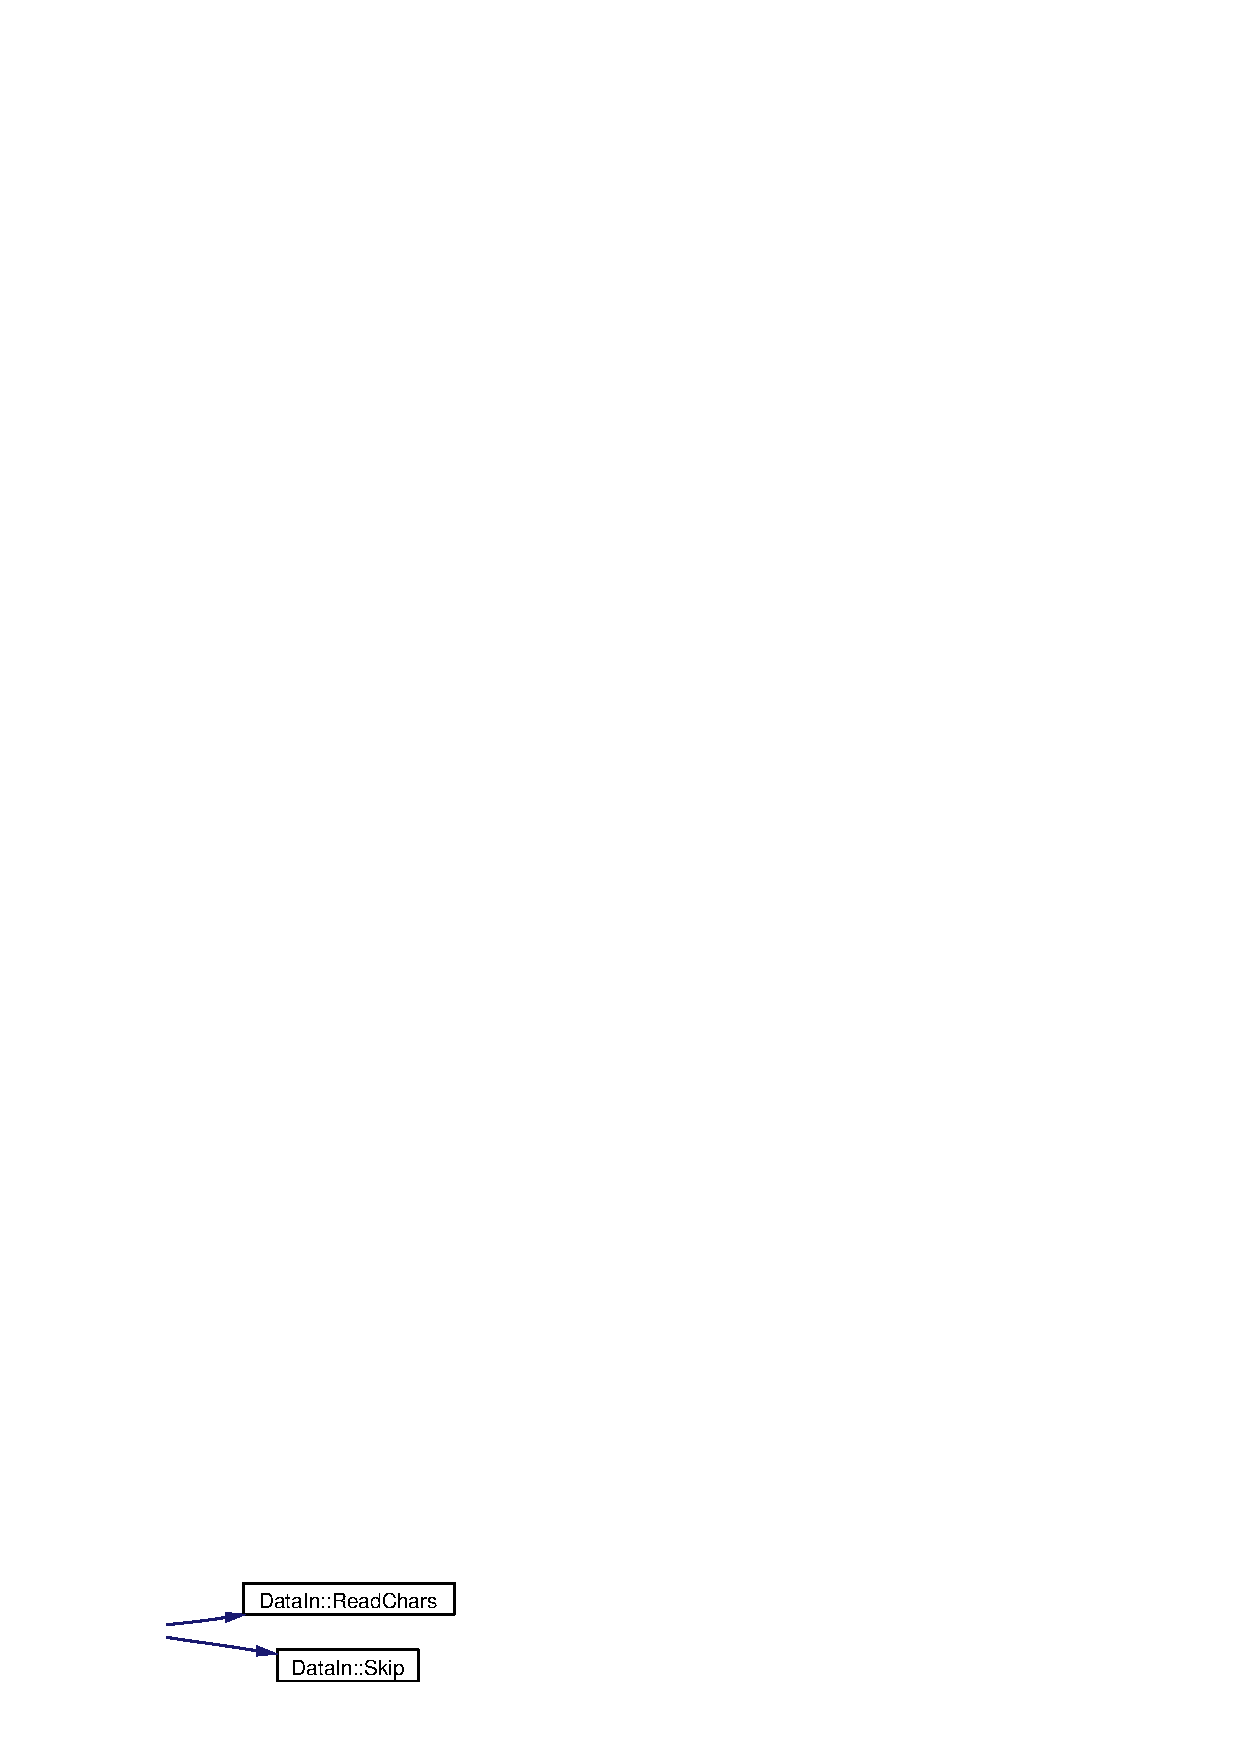
\includegraphics[width=113pt]{test_8cpp_a0_cgraph}
\end{center}
\end{figure}
